\subsection{Simulation in MCNP}

MCNP6 \cite{werner_mcnp_2017} was used to simulate gamma-ray spectra resulting from neutron activation of soil samples. Each simulation modeled a soil sample undergoing neutron activation with varying concentrations of carbon and other common soil constituents. The geometry was set up to mimic in situ measurement conditions, with a neutron source placed above a soil slab and a detector positioned to capture emitted gamma rays \cite{kavetskiy_neutron-stimulated_2017}.


In figure \ref{fig:mcnp_geometry}, the side view of the MCNP simulation setup is shown, highlighting the arrangement of the neutron source, soil slab, and detector. The geometry is designed to accurately represent the in situ conditions under which the soil samples are analyzed.

% \begin{figure}[H]
% \centering
% 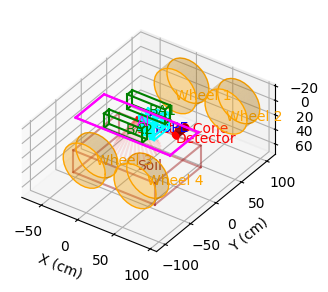
\includegraphics[width=0.8\textwidth]{../Figures/DataGeneration/MCNPGeometry.png}
% \caption{Geometry of MCNP simulation setup showing neutron source, soil slab, and detector configuration (Side View)}
% \label{fig:mcnp_geometry}
% \end{figure}

\begin{figure}[H]
\centering
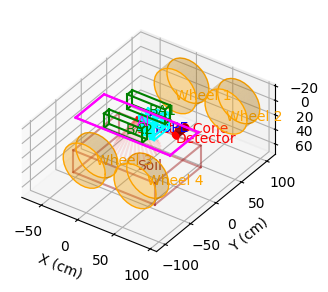
\includegraphics[width=0.8\textwidth,clip,trim=0cm 5cm 0cm 2cm]{../Figures/DataGeneration/MCNPGeometry.png}
\caption{Geometry of MCNP simulation setup showing neutron source, soil slab, and detector configuration (Side View)}
\label{fig:mcnp_geometry}
\end{figure}

In figure \ref{fig:mcnp_geometry_top}, the top view of the MCNP simulation setup is presented, providing a clear view of the spatial arrangement of the components, including the shielding around the detector to minimize background radiation.


\begin{figure}[H]
\centering
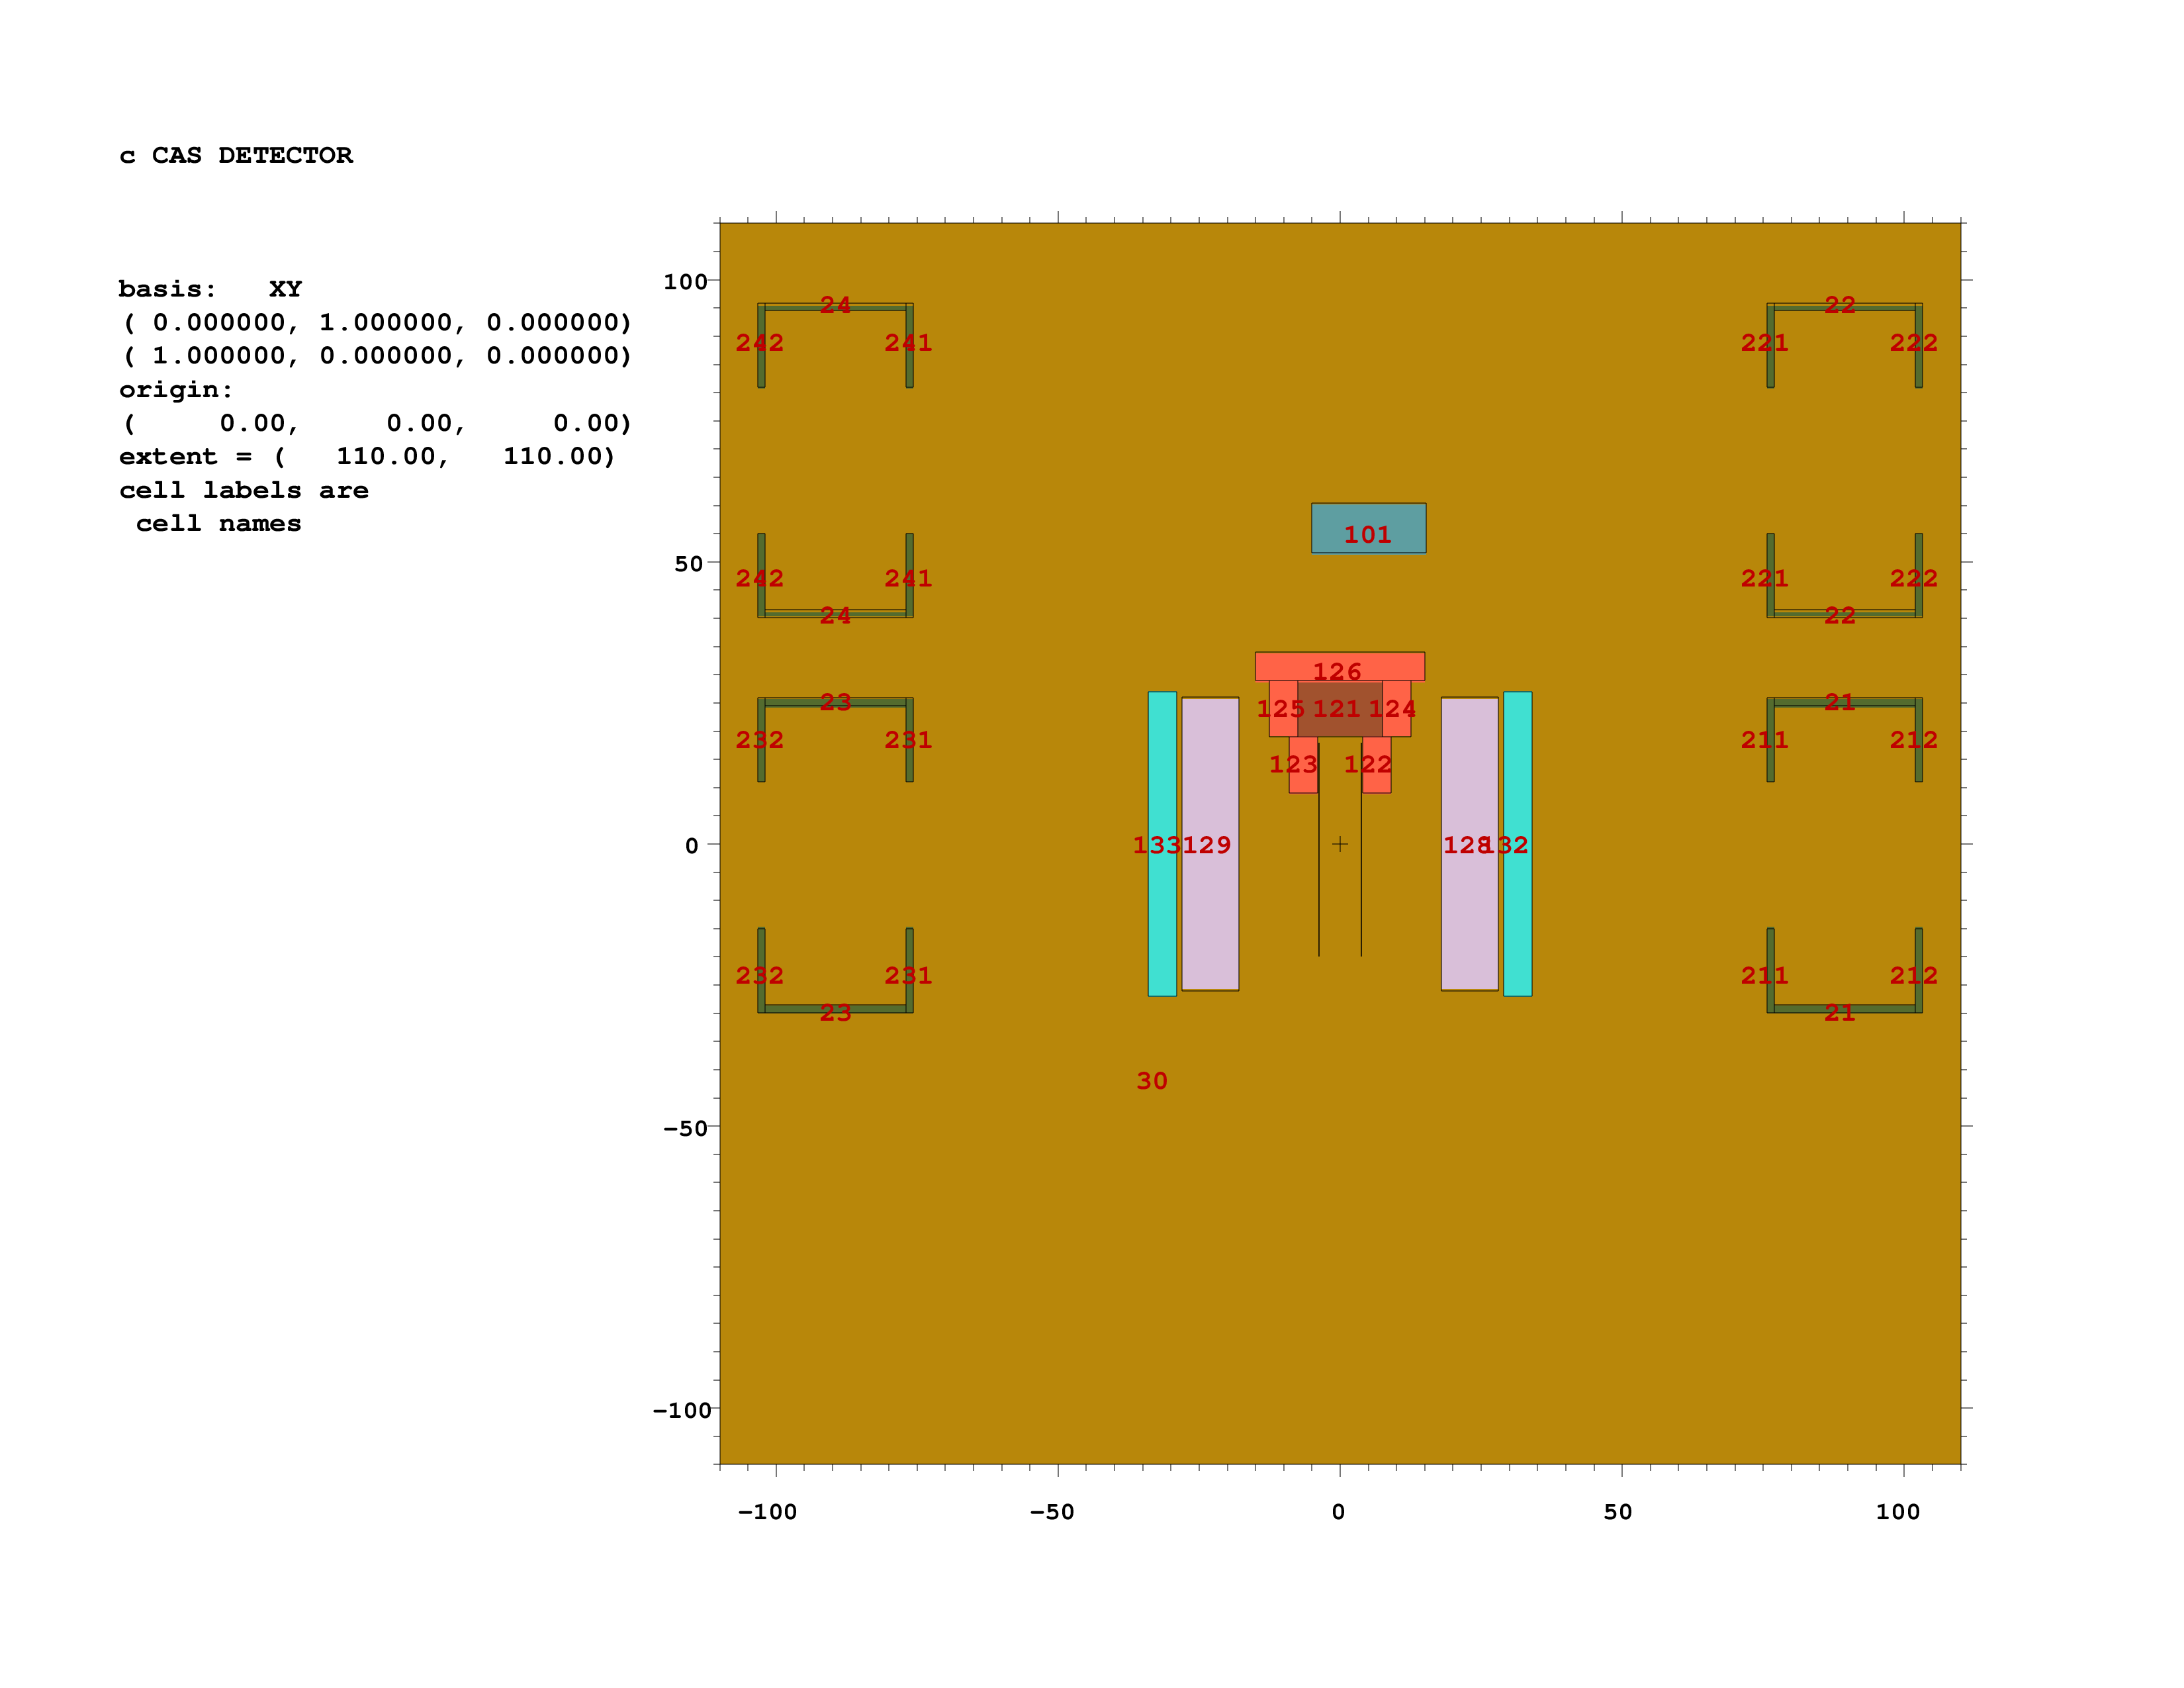
\includegraphics[width=0.8\textwidth]{../Figures/DataGeneration/top.png}
\caption{Cross section of MCNP simulation setup showing wheels and shielding (Top View)}
\label{fig:mcnp_geometry_top}
\end{figure}

Key simulation parameters included:
\begin{itemize}
\item \textbf{Neutron source energy:} API120 portable neutron (D-T generator) generator \cite{kavetskiy_energy_2018}
\item \textbf{Soil slab dimensions:} 112 cm × 90 cm × 30 cm
\item \textbf{Detector type:} NaI detector \cite{yakubova_measuring_2025}
\item \textbf{Tally:} F8 (pulse height tally) for gamma spectra
\end{itemize}

This approach enables the generation of realistic spectral data for a variety of soil compositions, forming the basis for evaluating different NGSA techniques. Table \ref{tab:chemical_identifiers} lists the MCNP chemical identifiers for the elements considered in the simulations.

\begin{table}[H]
    \centering
    \caption{MCNP Chemical Identifiers}
    \label{tab:chemical_identifiers}
    \begin{tabular}{lrrrrrrr}
    \hline
    Element         &    C &    H &    O &    Si &    Na &    Al &     K \\
    \hline
    MCNP Identifier & 6000 & 1001 & 8016 & 14000 & 11023 & 13027 & 19000 \\
    \hline
    \end{tabular}
\end{table}